% Created 2025-04-11 Fri 00:20
% Intended LaTeX compiler: pdflatex
\documentclass[presentation]{beamer}
\usepackage[utf8]{inputenc}
\usepackage[T1]{fontenc}
\usepackage{graphicx}
\usepackage{longtable}
\usepackage{wrapfig}
\usepackage{rotating}
\usepackage[normalem]{ulem}
\usepackage{amsmath}
\usepackage{amssymb}
\usepackage{capt-of}
\usepackage{hyperref}
\usepackage[slovene]{babel}
\usepackage[]{babel}
\usepackage{fvextra}
\usetheme{Dresden}
\author{Nikola Brković}
\date{\today}
\title{XMPP}
\hypersetup{
 pdfauthor={Nikola Brković},
 pdftitle={XMPP},
 pdfkeywords={},
 pdfsubject={},
 pdfcreator={Emacs 29.4 (Org mode 9.6.15)}, 
 pdflang={Slovene}}

% Setup for code blocks [1/2]

\usepackage{fvextra}

\fvset{%
  commandchars=\\\{\},
  highlightcolor=white!95!black!80!blue,
  breaklines=true,
  breaksymbol=\color{white!60!black}\tiny\ensuremath{\hookrightarrow}}

% Make line numbers smaller and grey.
\renewcommand\theFancyVerbLine{\footnotesize\color{black!40!white}\arabic{FancyVerbLine}}

\usepackage{xcolor}

% In case engrave-faces-latex-gen-preamble has not been run.
\providecolor{EfD}{HTML}{f7f7f7}
\providecolor{EFD}{HTML}{28292e}

% Define a Code environment to prettily wrap the fontified code.
\usepackage[breakable,xparse]{tcolorbox}
\DeclareTColorBox[]{Code}{o}%
{colback=EfD!98!EFD, colframe=EfD!95!EFD,
  fontupper=\footnotesize\setlength{\fboxsep}{0pt},
  colupper=EFD,
  IfNoValueTF={#1}%
  {boxsep=2pt, arc=2.5pt, outer arc=2.5pt,
    boxrule=0.5pt, left=2pt}%
  {boxsep=2.5pt, arc=0pt, outer arc=0pt,
    boxrule=0pt, leftrule=1.5pt, left=0.5pt},
  right=2pt, top=1pt, bottom=0.5pt,
  breakable}

% Support listings with captions
\usepackage{float}
\floatstyle{plain}
\newfloat{listing}{htbp}{lst}
\newcommand{\listingsname}{Listing}
\floatname{listing}{\listingsname}
\newcommand{\listoflistingsname}{List of Listings}
\providecommand{\listoflistings}{\listof{listing}{\listoflistingsname}}


% Setup for code blocks [2/2]: syntax highlighting colors

\newcommand\efstrut{\vrule height 2.1ex depth 0.8ex width 0pt}
\definecolor{EFD}{HTML}{000000}
\definecolor{EfD}{HTML}{ffffff}
\newcommand{\EFD}[1]{\textcolor{EFD}{#1}} % default
\definecolor{EFvp}{HTML}{000000}
\newcommand{\EFvp}[1]{\textcolor{EFvp}{#1}} % variable-pitch
\definecolor{EFh}{HTML}{7f7f7f}
\newcommand{\EFh}[1]{\textcolor{EFh}{#1}} % shadow
\definecolor{EFsc}{HTML}{228b22}
\newcommand{\EFsc}[1]{\textcolor{EFsc}{\textbf{#1}}} % success
\definecolor{EFw}{HTML}{ff8e00}
\newcommand{\EFw}[1]{\textcolor{EFw}{\textbf{#1}}} % warning
\definecolor{EFe}{HTML}{ff0000}
\newcommand{\EFe}[1]{\textcolor{EFe}{\textbf{#1}}} % error
\definecolor{EFl}{HTML}{ff0000}
\newcommand{\EFl}[1]{\textcolor{EFl}{#1}} % link
\definecolor{EFlv}{HTML}{ff0000}
\newcommand{\EFlv}[1]{\textcolor{EFlv}{#1}} % link-visited
\definecolor{EFhi}{HTML}{ff0000}
\newcommand{\EFhi}[1]{\textcolor{EFhi}{#1}} % highlight
\definecolor{EFc}{HTML}{b22222}
\newcommand{\EFc}[1]{\textcolor{EFc}{#1}} % font-lock-comment-face
\definecolor{EFcd}{HTML}{b22222}
\newcommand{\EFcd}[1]{\textcolor{EFcd}{#1}} % font-lock-comment-delimiter-face
\definecolor{EFs}{HTML}{8b2252}
\newcommand{\EFs}[1]{\textcolor{EFs}{#1}} % font-lock-string-face
\definecolor{EFd}{HTML}{8b2252}
\newcommand{\EFd}[1]{\textcolor{EFd}{#1}} % font-lock-doc-face
\definecolor{EFm}{HTML}{008b8b}
\newcommand{\EFm}[1]{\textcolor{EFm}{#1}} % font-lock-doc-markup-face
\definecolor{EFk}{HTML}{9370db}
\newcommand{\EFk}[1]{\textcolor{EFk}{#1}} % font-lock-keyword-face
\definecolor{EFb}{HTML}{483d8b}
\newcommand{\EFb}[1]{\textcolor{EFb}{#1}} % font-lock-builtin-face
\definecolor{EFf}{HTML}{0000ff}
\newcommand{\EFf}[1]{\textcolor{EFf}{#1}} % font-lock-function-name-face
\definecolor{EFv}{HTML}{a0522d}
\newcommand{\EFv}[1]{\textcolor{EFv}{#1}} % font-lock-variable-name-face
\definecolor{EFt}{HTML}{228b22}
\newcommand{\EFt}[1]{\textcolor{EFt}{#1}} % font-lock-type-face
\definecolor{EFo}{HTML}{008b8b}
\newcommand{\EFo}[1]{\textcolor{EFo}{#1}} % font-lock-constant-face
\definecolor{EFwr}{HTML}{ff0000}
\newcommand{\EFwr}[1]{\textcolor{EFwr}{\textbf{#1}}} % font-lock-warning-face
\newcommand{\EFnc}[1]{#1} % font-lock-negation-char-face
\definecolor{EFpp}{HTML}{483d8b}
\newcommand{\EFpp}[1]{\textcolor{EFpp}{#1}} % font-lock-preprocessor-face
\newcommand{\EFrc}[1]{\textbf{#1}} % font-lock-regexp-grouping-construct
\newcommand{\EFrb}[1]{\textbf{#1}} % font-lock-regexp-grouping-backslash
\newcommand{\EFob}[1]{#1} % org-block
\newcommand{\EFobb}[1]{#1} % org-block-begin-line
\newcommand{\EFobe}[1]{#1} % org-block-end-line
\definecolor{EFOa}{HTML}{0000ff}
\newcommand{\EFOa}[1]{\textcolor{EFOa}{#1}} % outline-1
\definecolor{EFOb}{HTML}{a0522d}
\newcommand{\EFOb}[1]{\textcolor{EFOb}{#1}} % outline-2
\definecolor{EFOc}{HTML}{a020f0}
\newcommand{\EFOc}[1]{\textcolor{EFOc}{#1}} % outline-3
\definecolor{EFOd}{HTML}{b22222}
\newcommand{\EFOd}[1]{\textcolor{EFOd}{#1}} % outline-4
\definecolor{EFOe}{HTML}{228b22}
\newcommand{\EFOe}[1]{\textcolor{EFOe}{#1}} % outline-5
\definecolor{EFOf}{HTML}{008b8b}
\newcommand{\EFOf}[1]{\textcolor{EFOf}{#1}} % outline-6
\definecolor{EFOg}{HTML}{483d8b}
\newcommand{\EFOg}[1]{\textcolor{EFOg}{#1}} % outline-7
\definecolor{EFOh}{HTML}{8b2252}
\newcommand{\EFOh}[1]{\textcolor{EFOh}{#1}} % outline-8
\definecolor{EFhn}{HTML}{008b8b}
\newcommand{\EFhn}[1]{\textcolor{EFhn}{#1}} % highlight-numbers-number
\definecolor{EFhq}{HTML}{9370db}
\newcommand{\EFhq}[1]{\textcolor{EFhq}{#1}} % highlight-quoted-quote
\definecolor{EFhs}{HTML}{008b8b}
\newcommand{\EFhs}[1]{\textcolor{EFhs}{#1}} % highlight-quoted-symbol
\definecolor{EFrda}{HTML}{707183}
\newcommand{\EFrda}[1]{\textcolor{EFrda}{#1}} % rainbow-delimiters-depth-1-face
\definecolor{EFrdb}{HTML}{7388d6}
\newcommand{\EFrdb}[1]{\textcolor{EFrdb}{#1}} % rainbow-delimiters-depth-2-face
\definecolor{EFrdc}{HTML}{909183}
\newcommand{\EFrdc}[1]{\textcolor{EFrdc}{#1}} % rainbow-delimiters-depth-3-face
\definecolor{EFrdd}{HTML}{709870}
\newcommand{\EFrdd}[1]{\textcolor{EFrdd}{#1}} % rainbow-delimiters-depth-4-face
\definecolor{EFrde}{HTML}{907373}
\newcommand{\EFrde}[1]{\textcolor{EFrde}{#1}} % rainbow-delimiters-depth-5-face
\definecolor{EFrdf}{HTML}{6276ba}
\newcommand{\EFrdf}[1]{\textcolor{EFrdf}{#1}} % rainbow-delimiters-depth-6-face
\definecolor{EFrdg}{HTML}{858580}
\newcommand{\EFrdg}[1]{\textcolor{EFrdg}{#1}} % rainbow-delimiters-depth-7-face
\definecolor{EFrdh}{HTML}{80a880}
\newcommand{\EFrdh}[1]{\textcolor{EFrdh}{#1}} % rainbow-delimiters-depth-8-face
\definecolor{EFrdi}{HTML}{887070}
\newcommand{\EFrdi}[1]{\textcolor{EFrdi}{#1}} % rainbow-delimiters-depth-9-face
\definecolor{EFany}{HTML}{CDCD00}
\newcommand{\EFany}[1]{\textcolor{EFany}{#1}} % ansi-color-yellow
\definecolor{EFanr}{HTML}{CD0000}
\newcommand{\EFanr}[1]{\textcolor{EFanr}{#1}} % ansi-color-red
\definecolor{EFanb}{HTML}{000000}
\newcommand{\EFanb}[1]{\textcolor{EFanb}{#1}} % ansi-color-black
\definecolor{EFang}{HTML}{00CD00}
\newcommand{\EFang}[1]{\textcolor{EFang}{#1}} % ansi-color-green
\definecolor{EFanB}{HTML}{0000EE}
\newcommand{\EFanB}[1]{\textcolor{EFanB}{#1}} % ansi-color-blue
\definecolor{EFanc}{HTML}{00CDCD}
\newcommand{\EFanc}[1]{\textcolor{EFanc}{#1}} % ansi-color-cyan
\definecolor{EFanw}{HTML}{E5E5E5}
\newcommand{\EFanw}[1]{\textcolor{EFanw}{#1}} % ansi-color-white
\definecolor{EFanm}{HTML}{CD00CD}
\newcommand{\EFanm}[1]{\textcolor{EFanm}{#1}} % ansi-color-magenta
\definecolor{EFANy}{HTML}{EEEE00}
\newcommand{\EFANy}[1]{\textcolor{EFANy}{#1}} % ansi-color-bright-yellow
\definecolor{EFANr}{HTML}{EE0000}
\newcommand{\EFANr}[1]{\textcolor{EFANr}{#1}} % ansi-color-bright-red
\newcommand{\EFANb}[1]{#1} % ansi-color-bright-black
\definecolor{EFANg}{HTML}{00EE00}
\newcommand{\EFANg}[1]{\textcolor{EFANg}{#1}} % ansi-color-bright-green
\definecolor{EFANB}{HTML}{0000FF}
\newcommand{\EFANB}[1]{\textcolor{EFANB}{#1}} % ansi-color-bright-blue
\definecolor{EFANc}{HTML}{00EEEE}
\newcommand{\EFANc}[1]{\textcolor{EFANc}{#1}} % ansi-color-bright-cyan
\newcommand{\EFANw}[1]{#1} % ansi-color-bright-white
\newcommand{\EFANm}[1]{#1} % ansi-color-bright-magenta
\begin{document}

\maketitle

\section{Namen in arhitektura protokola}
\label{sec:org43ecd96}

\begin{frame}[label={sec:orgccea582}]{Namen protokola}
\begin{itemize}
\item \emph{Extensible Messaging and Presence Protocol}
\item "Protokol, namenjen izmenjavi strukturiranih podatkov v približno
realnem času med dvema ali več entitetami"
\item V praksi predvsem hipno sporočanje (\emph{Instant Messaging})
\end{itemize}
\end{frame}

\begin{frame}[label={sec:orgdb242ce}]{Arhitektura protokola}
\begin{itemize}
\item Zgled: SMTP
\item Porazdeljeno omrežje
\item Vloge:
\begin{itemize}
\item strežnik
\item uporabnik
\item (vir)
\end{itemize}
\end{itemize}
\end{frame}

\begin{frame}[label={sec:orga10567c},fragile]{Arhitektura protokola}
 \begin{itemize}
\item Identifikator: JID (\emph{Jabber ID})
\item Strežnik: JID je enak domeni (\texttt{jabber.si})
\item Uporabnik: \texttt{<uporabnik>@<strežnik>} (\texttt{julija@jabber.si})
\item Vir: \texttt{<uporabnik>@<strežnik>/<vir>} (\texttt{julija@jabber.si/prenosnik})
\end{itemize}
\end{frame}

\section{Scenarij komunikacije}
\label{sec:orgd6a8cb5}

\begin{frame}[label={sec:org3fb5006}]{Lokalni uporabniki}
\begin{figure}[H]
\centering
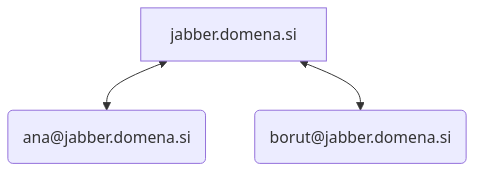
\includegraphics[width=.9\linewidth]{images/local-server.png}
\caption{\label{fig:org3e789db}Komunikacija med uporabniki na istem strežniku}
\end{figure}
\end{frame}

\begin{frame}[label={sec:orge1a6f66}]{Oddaljeni uporabniki}
\begin{figure}[H]
\centering

\includegraphics[width=.9\linewidth]{images/cross-server.png}
\caption{\label{fig:orgeb5874d}Komunikacija med uporabniki na različnih strežnikih}
\end{figure}
\end{frame}

\section{Opis specifikacije}
\label{sec:orgf16b136}

\begin{frame}[label={sec:orgb116f60}]{Opis specifikacije}
\begin{itemize}
\item \href{https://datatracker.ietf.org/doc/rfc6120/}{Extensible Messaging and Presence Protocol (XMPP): Core} (XMPP-CORE)
\item \href{https://datatracker.ietf.org/doc/rfc6121/}{Extensible Messaging
and Presence Protocol (XMPP): Instant Messaging and Presence}
(XMPP-IM)
\item \href{https://datatracker.ietf.org/doc/rfc7622/}{Extensible Messaging and Presence Protocol (XMPP): Address Format}
(XMPP-ADDR)
\item Razširitve (XEP)
\end{itemize}
\end{frame}

\begin{frame}[label={sec:org2dfbaca},fragile]{XMPP-CORE}
 \begin{itemize}
\item Povezava po TCP: tok XML
\item Posamezno sporočilo: stanca XML
\item Vrste sporočil: \texttt{<message/>}, \texttt{<presence/>}, \texttt{<iq/>}
\item Omogoča TLS ali SASL
\end{itemize}
\end{frame}

\begin{frame}[label={sec:orga1eb00d},fragile]{XMPP-IM}
 \begin{itemize}
\item Klepetalne seje (\texttt{chat} ali \texttt{groupchat})
\item Spisek (\emph{roster})
\item Naročanje na prisotnost
\end{itemize}
\end{frame}

\begin{frame}[label={sec:org7b82a12}]{XMPP-ADDR}
\begin{itemize}
\item Kodiranje črk, ki so del kodirnega sistema Unicode
\end{itemize}
\end{frame}

\begin{frame}[label={sec:orgbc13993}]{Razširitve}
\begin{itemize}
\item \href{https://xmpp.org/extensions/xep-0045.html}{Multi-User Chat (XEP-0045)} - podrobneje določa delovanje skupinskih
klepetov, ki so omenjeni že v XMPP-IM (Saint-Andre, Peter, 2002),
\item \href{https://xmpp.org/extensions/xep-0166.html}{Jingle (XEP-0166)} - omogoča dogovarjanje med entitetami preko XMPP
za neposredne medijske seje, ki potekajo po nekem drugem
kanalu. Uporablja se predvsem za glasovne ali video
klepete. (Ludwig, Scott and Beda, Joe and Saint-Andre, Peter and McQueen, Robert and Egan, Sean and Hildebrand, Joe, 2005)
\item \href{https://xmpp.org/extensions/xep-0234.html}{Jingle File Transfer (XEP-0234)} - določa format seje Jingle za
prenos datotek (Saint-Andre, Peter and Stout, Lance, 2008)
\end{itemize}
\end{frame}

\section{Format sporočil}
\label{sec:orgf41f4a2}

\begin{frame}[label={sec:org86e2948},fragile]{Message}
 \begin{Code}
\begin{Verbatim}
\color{EFD}<\textcolor[HTML]{0000ff}{message} \textcolor[HTML]{a0522d}{from}=\EFs{'france@jabber.si/hiša'}
            \textcolor[HTML]{a0522d}{id}=\EFs{'ju2ba41c'}
            \textcolor[HTML]{a0522d}{to}=\EFs{'julija@jabber.si'}
            \textcolor[HTML]{a0522d}{type}=\EFs{'chat'}
            \textcolor[HTML]{483d8b}{xml}:\textcolor[HTML]{a0522d}{lang}=\EFs{'si'}>
  <\textcolor[HTML]{0000ff}{body}>
    Sijalo sonce je podobe zale,
    pogleda tvojga pil sem žarke mile,
    ljubezni so cvetlice kal pognale.
  </\textcolor[HTML]{0000ff}{body}>
</\textcolor[HTML]{0000ff}{message}>
\end{Verbatim}
\end{Code}

(Prešeren, France, 1999)
\end{frame}

\begin{frame}[label={sec:org2cbe184},fragile]{Presence}
 \begin{Code}
\begin{Verbatim}
\color{EFD}<\textcolor[HTML]{0000ff}{presence} \textcolor[HTML]{483d8b}{xml}:\textcolor[HTML]{a0522d}{lang}=\EFs{'si'}>
  <\textcolor[HTML]{0000ff}{show}>away</\textcolor[HTML]{0000ff}{show}>
  <\textcolor[HTML]{0000ff}{status}>
    Oblak ne ve, in val ne kam,
    kam nese me obup, ne znam.
  </\textcolor[HTML]{0000ff}{status}>
</\textcolor[HTML]{0000ff}{presence}>
\end{Verbatim}
\end{Code}

(Prešeren, France, 1999)
\end{frame}

\begin{frame}[label={sec:org974c2f8},fragile]{IQ (Info/Query)}
 Zahteva za pridobivanje spiska

\begin{Code}
\begin{Verbatim}
\color{EFD}<\textcolor[HTML]{0000ff}{iq} \textcolor[HTML]{a0522d}{from}=\EFs{'france@jabber.si/hiša'}
    \textcolor[HTML]{a0522d}{id}=\EFs{'bv1bs71f'}
    \textcolor[HTML]{a0522d}{type}=\EFs{'get'}>
  <\textcolor[HTML]{0000ff}{query} \textcolor[HTML]{483d8b}{xmlns}=\EFs{'jabber:iq:roster'}/>
</\textcolor[HTML]{0000ff}{iq}>
\end{Verbatim}
\end{Code}
\end{frame}

\begin{frame}[label={sec:org60cf44c},fragile]{IQ (Info/Query)}
 Odgovor strežnika na zahtevo

\begin{Code}
\begin{Verbatim}
\color{EFD}<\textcolor[HTML]{0000ff}{iq} \textcolor[HTML]{a0522d}{id}=\EFs{'bv1bs71f'}
       \textcolor[HTML]{a0522d}{to}=\EFs{'france@jabber.si/hiša'}
       \textcolor[HTML]{a0522d}{type}=\EFs{'result'}>
    <\textcolor[HTML]{0000ff}{query} \textcolor[HTML]{483d8b}{xmlns}=\EFs{'jabber:iq:roster'} \textcolor[HTML]{a0522d}{ver}=\EFs{'ver7'}>
      <\textcolor[HTML]{0000ff}{item} \textcolor[HTML]{a0522d}{jid}=\EFs{'matija@jabber.si'}/>
      <\textcolor[HTML]{0000ff}{item} \textcolor[HTML]{a0522d}{jid}=\EFs{'julija@xmpp.si'}/>
    </\textcolor[HTML]{0000ff}{query}>
  </\textcolor[HTML]{0000ff}{iq}>
\end{Verbatim}
\end{Code}
\end{frame}

\section{Literatura}
\label{sec:org15a6bd0}

\begin{frame}[label={sec:org6e8e701}]{Literatura}
\noindent
Ludwig, Scott and Beda, Joe and Saint-Andre, Peter and McQueen, Robert and Egan, Sean and Hildebrand, Joe (2005). \emph{Jingle}, XMPP Standards Foundation.

\noindent
Prešeren, France (1999). \emph{Poezije}, Mladinska knjiga.

\noindent
Saint-Andre, Peter (2002). \emph{Multi-User Chat}, XMPP Standards Foundation.

\noindent
Saint-Andre, Peter and Stout, Lance (2008). \emph{Jingle File Transfer}, XMPP Standards Foundation.
\end{frame}
\end{document}
